Here, we propose a hybrid adaptive large neighborhood search algorithm for solving the problem described in the previous chapter. Next, we describe the methodology for evaluation of the proposed algorithm. Lastly, we illustrate the implementation of all mentioned parts.

\section{The Algorithm for the PDPTW} \label{sec:halns}

    The adaptive large neighborhood search (ALNS) algorithm has been successfully applied to a wide range of VRP problems, including PDPTW and DARP. In addition, the robustness of ALNS allows to efficiently solve problems with different features. However, ALNS is prone to get trapped in local optima when applied to highly constrained problems. Therefore, in this study, we combine diverse intensification strategies in the promising regions of the solution space as well as several diversification techniques to direct the search towards new and unexplored regions of the solution space. The algorithm used in this thesis is a hybrid version of ALNS, named \emph{hybrid adaptive large neighborhood search} (HALNS) and is based on the research made on DARP by primarily Masmoudi et al. (2020) \cite{Masmoudi2020}, and others, including Ropke and Pisinger (2006) \cite{Ropke2006}, Gschwind and Drexl (2016) \cite{Gschwind2016}, and Masmoudi et al. (2016) \cite{Masmoudi2016}.
    
    The majority of the ALNS algorithms in the literature uses the following approach for restarting the search: when a new solution is not better than the current solution, and is not accepted using the acceptance criterion known from the simulated annealing algorithm, the ALNS algorithm restarts the search from a solution that is generated from the same current solution by applying the removal and insertion operators. However, our algorithm does not return to the current solution. Instead, it generates a new solution using a crossover operator known from genetic algorithms. It combines the current best solution with the new solution generated by the constructive heuristics used for obtaining the initial solution. This solution is then used as the current solution. This approach gives the algorithm more diversification power as this newly generated solution is placed in a new region of the solution space, thanks to the crossover.
    
        \begin{algorithm}[!ht]
    \Input{Instance of PDPTW consisting of a set of requests and required number of drivers.}
    $ x \leftarrow InitialSolution(instance) $ \tcc*{current solution}
    $ x_{\mathrm{best}} \leftarrow x $ \tcc*{best solution}
    $ \tau \leftarrow \tau_{\mathrm{max}} $ \tcc*{temperature}
    Initialize the weights of insertion, removal, and local search operators\;
    \For{$ i \in 1,\ldots,i_{\mathrm{max}} $} {
        $x' \leftarrow$ apply removal to the current solution $ x $\;
        $x_{\mathrm{new}} \leftarrow$ apply insertion to $ x' $ \tcc*{new solution}
        
        \If{$x_{\mathrm{new}}$ is feasible} {
            \If{$cost(x_{\mathrm{new}}) < cost(x)$ or $cost(x_{\mathrm{new}})$ satisfies acceptance criterion} {
                $x \leftarrow x_{\mathrm{new}}$\;
            }
            \ElseIf{$cost(x_{\mathrm{new}}) > cost(x)$} {
                $ x_{\mathrm{init}} \leftarrow InitialSolution(instance) $\;
                $ x \leftarrow Crossover(x_{\mathrm{best}}, x_{\mathrm{init}}) $\;
            }
            \If{$cost(x_{\mathrm{new}}) < cost(x_{\mathrm{best}})$} {
                $x_{\mathrm{best}} \leftarrow x_{\mathrm{new}}$\;
                $\tau_{\mathrm{best}} \leftarrow \tau$\;
            }
            \ElseIf{$cost(x_{\mathrm{new}}) < cost(x_{\mathrm{best}})(1+\delta)$} {
                $x_{\mathrm{new}} \leftarrow LocalSearch(x_{\mathrm{new}})$\;
                \If{$cost(x_{\mathrm{new}}) < cost(x_{\mathrm{best}})$} {
                    $x_{\mathrm{best}} \leftarrow x_{\mathrm{new}}$\;
                    $\tau_{\mathrm{best}} \leftarrow \tau$\;
                }
            }
        }
        $\tau \leftarrow \alpha \tau$\;
        \If{$\tau < 0.01$} {
            $\tau_{\mathrm{best}} \leftarrow 2\tau_{\mathrm{best}}$\;
            $\tau \leftarrow min(\tau_{\mathrm{best}}, \tau_{\mathrm{max}})$\;
        }
        update the weights of insertion, removal and local search operators\;
    }
    \Return{$x_{\mathrm{best}}$}
    \caption{\label{alg:halns-loop} Hybrid Adaptive Large Neighborhood Search for PDPTW}
    \end{algorithm}
    
    
    
    Additionally, in most ALNS approaches, the best solution is updated only if the newly generated solution is better than the best solution. On the contrary, our algorithm uses an acceptance function for the new solution, which works as follows: if the newly generated solution is not worse than $\delta\,\%$ from the best solution, the new solution is not discarded. Rather, this solution is intensified using the local search procedure (see section \ref{halns:local-search}), and then compared with the best solution again. The better of the two solutions becomes the new best solution. This approach gives more chance for promising solutions to become new best solutions and thus results in more diversification power. On the other hand, using the local search procedure for promising solutions results in intensifying the search towards even better solutions.
    
    These strategies form our hybrid adaptive large neighborhood search, which combines the diversification ability of the crossover procedure and the modified acceptance function with the intensification ability of the local search procedure. Although similar approaches have been used to solve the DARP by Masmoudi et al. (2020) \cite{Masmoudi2020}, to the best of our knowledge, these novel techniques have not yet been applied to the food delivery planning problem.
    
    The main loop of our HALNS algorithm is outlined in algorithm \ref{alg:halns-loop}. Similarly to the ALNS known from Ropke and Pisinger (2006) \cite{Ropke2006}, Gschwind and Drexl (2016) \cite{Gschwind2016}, and Masmoudi et al. (2016) \cite{Masmoudi2016}, the algorithm keeps track of (1) the best solution found so far $x_{\mathrm{best}}$, (2) the current solution $x$ and (3) the newly generated solution $x_{\mathrm{new}}$. The algorithm is executed for a specified number of iterations $i_{\mathrm{max}}$ to find the best solution $x_{\mathrm{best}}$ based on its cost $cost(x_{\mathrm{best}})$ (see section \ref{halns:cost}). 
    
    In the beginning, the current solution $x$ is initialized to the new solution obtained by the construction heuristics (see section \ref{halns:init-solution}). Best solution $x_{\mathrm{best}}$ is set to the value of current solution $x$. We also initialize the temperature $\tau$ to the value $\tau_{\mathrm{max}}$ and we initialize the weights of insertion, removal, and local search operators for the adaptive weight adjustment, further described in section \ref{halns:weight}.
    
    In each iteration of the algorithm, the new solution $x_{\mathrm{new}}$ is generated from the current solution $x$ by applying the removal and insertion operators, which are described in section \ref{halns:insertion-removal}. If the best solution $x_{\mathrm{best}}$ was improved in the last iteration, one removal and one insertion operator are used to generate $x_{\mathrm{new}}$. Elseways, two removal operators and one insertion operator are used to further diversify the search. Our removal operators destroy the current solution by removing a number of requests, whereas the insertion operators repair the solution by embeding all unplanned requests back to the solution. The specific removal and insertion operators are selected based on their past performance. The selection mechanism is further described in section \ref{halns:weight}. 
    
    The new solution $x_{\mathrm{new}}$ is accepted if it is better than the current solution $x$ or if it satisfies the acceptance criterion, i.e., we accept it with probability $e^{\big(cost(x_{\mathrm{new}}) - cost(x)\big)/\tau}$. Otherwise, a new solution is obtained by utilizing a randomly selected crossover operator (see section \ref{halns:diversification}) that combines the current best solution $x_{\mathrm{best}}$ with a new solution obtained from the constructive heuristics $x_{\mathrm{init}}$ (see section \ref{halns:init-solution}). If the cost of the new solution $cost(x_{\mathrm{new}})$ is lower than the cost of the current best solution $cost(x_{\mathrm{best}})$, $x_{\mathrm{new}}$ becomes the new $x_{\mathrm{best}}$. Else, if $cost(x_{\mathrm{new}})$ is worse than $x_{\mathrm{best}}$ by a maximum of $\delta\,\%$, $x_{\mathrm{new}}$ is improved with the local search and becomes the new best solution $x_{\mathrm{best}}$ if it has lower cost compared to $x_{\mathrm{best}}$ after the intensification of the local search procedure.
    
    The temperature $\tau$, used in the acceptance criterion, is decreased in each iteration by multiplying it with the cooling rate $\alpha$. If after the cooling procedure, the temperature value becomes lower than $0.01$, $\tau_{\mathrm{best}}$, used to record the temperature when $x_{\mathrm{best}}$ is found, is multiplied by $2$ and the value of $\tau$ is set to the value of $\tau_{\mathrm{best}}$. To make sure that the search does not start from scratch from a random solution, the temperature $\tau$ is limited to $\tau_{\mathrm{max}}$.
    
    \subsection{Cost Function} \label{halns:cost}
    
    The cost function is an essential part of our HALNS algorithm as it determines the quality of the produced solution. As the costs of the intermediate solutions are measured several times in each iteration of the algorithm, especially during the application of insertion operators and our constructive heuristics, the cost function needs to be reasonably fast. Our objective is to minimize the divergence from the defined time windows and the total distance driven by the vehicles.
    
    Sometimes, it may be beneficial for the driver to arrive at the customer location before the start of the time window so that he has a lower delay for the upcoming customers. However, computing the ideal times of arrival in the plan when allowing visiting the nodes before the earliest time set by the customer would increase the complexity of the whole algorithm. To overcome this issue, we do not allow to start a service on a node before its time window starts. As a result, when the driver arrives too soon at the location, he must wait until the time window starts to begin the service\footnote{In practice, the driver may serve the customer sooner and use that extra time to compensate later delays, for example due to traffic.}.
    
    A solution $x$ consists of a set of routes $E = \{e_0,\cdots,e_k\}$, where $k$ is the number of drivers. The cost function of a single route $e \in E$ is computed as $cost(e) = \beta t^{\mathrm{delay}}_e + \gamma t^{\mathrm{distance}}_e$, where $t^{\mathrm{delay}}_e$ is the total delay of the route $e$ in seconds, $t^{\mathrm{distance}}_e$ is the total travelled distance of the route $e$ in meters, and $\beta$ and $\gamma$ are the global parameters of the algorithm (see section \ref{halns:parameters}).
    
    The total delay is computed as:
    \[ t^{\mathrm{delay}}_e = \sum_{i = 1}^{|e|-1} \max\{t^{\mathrm{eta}}_i + t^{\mathrm{service}}_i + t^{\mathrm{travel}}_{i,i+1} - w^e_{i+1}, 0\} \]
    where $t^{\mathrm{eta}}_i$ is the expected time of arrival to node $i$, $t^{\mathrm{service}}_i$ is the service time at node $i$, $t^{\mathrm{travel}}_{i,j}$ is the travel time from node $i$ to node $j$, and finally $w^e_i$ is the end of the time window of node $i$.
    
    The total distance is computed as:
    \[ t^{\mathrm{distance}}_e = \sum_{i = 1}^{|e|-1} m_{i, i+1}\]
    where $m_{i, j}$ is the travel distance between nodes $i$ and $j$.
    
    The cost of the solution $x$ is calculated as the sum of the costs of all routes, i.e., $cost(x) = \sum_{k \in K} cost(e_k)$, where $K$ is the set of drivers and $e_k$ is the route of driver $k$.

    Figure \ref{fig:plan-traversal} shows an example of traversing a single route of five nodes to compute its cost. The driver arrives at nodes 1, 3, and 5 too soon and begins the service at the start of the time window. At node 4, the driver arrives late and the difference between the end of the time window and the arrival time is the delay that is added to the total cost.
    
    \begin{figure}[ht]
        \centering
        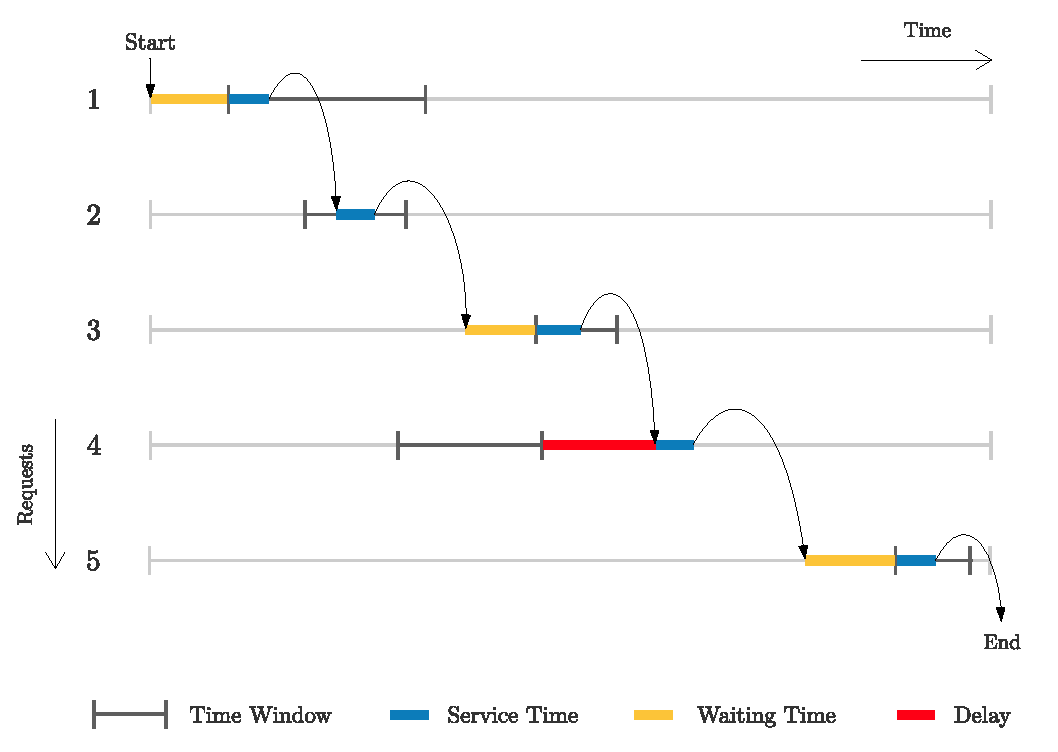
\includegraphics[width=1\textwidth]{figures/plan-traversal.pdf}
        \caption{An example of a single plan traversal for computing the cost function.}
        \label{fig:plan-traversal}
    \end{figure}
    
    
    \subsection{Removal and Insertion Operators} \label{halns:insertion-removal}
    
    The removal operators are used in each iteration to destroy the current solution by removing a number of requests from the solution and putting these requests into a set $R$. The insertion operators then repair the solution by taking the requests from the set $R$ and inserting them back into the solution, such that the solution is feasible.
    
    The removal and insertion operators were adopted from the existing literature, such as Ropke and Pisinger (2006) \cite{Ropke2006}, Pisinger and Ropke (2007) \cite{Pisinger2007}, and Demir et al. (2012) \cite{Demir2012} and adapted to our specific problem definition. The operators used in our version of HALNS are:
    
    \begin{description}
    		
    		\item [Random Request Removal (R1)] This operator randomly selects $n$ requests from the current solution $x$ and removes the corresponding pickup and drop-off nodes forming a new solution $x'$.
    		
    		\item [Path Removal (R2)] Similar to the removal operator presented by Demir et al. (2012) \cite{Demir2012}, our path removal operator randomly selects one request $r$ from the current solution $x$ and removes $n$ nodes in the plan between the pickup node $p_r$ and drop-off node $d_r$ of request $r$. We also remove all corresponding nodes such that we always remove the whole request. In other words, when only a pickup node is to be removed, we also remove the drop-off node of the same request even if it is outside of the $p_r$ and $d_r$ path.
    		
    		\item [Related Removal (R3)] This operator, based on Ropke and Pisinger (2006) \cite{Ropke2006}, randomly selects one request $r$ in the current solution and removes $n$ most related requests. The function which defines how much two requests $i$ and $j$ are related is defined as follows: $R(i,j) = m_{p_i, p_j} + m_{d_i, d_j} + \rho(|t^{\mathrm{eta}}_{p_i} - t^{\mathrm{eta}}_{p_j}| + |t^{\mathrm{eta}}_{d_i} - t^{\mathrm{eta}}_{d_j}|)$, where $p_i$ and $p_j$ (or $d_i$ and $d_j$) are the pickup nodes (or the drop-off nodes) of requests $i$ and $j$, respectively; $m_{i,j}$ is the distance between two nodes; $t^{\mathrm{eta}}_i$ is the expected time of arrival to the node $i$ in the current plan; and $\rho \in [0,1]$ is a control parameter. The operator then sorts the unplanned requests based on the function $R$ and removes $n$ requests in this order forming a new solution $x'$.
    		
    		\item [Time-oriented Removal (R4)] This operator is a special case of the related removal operator R3, where the requests that are serviced in similar times are removed. In this case, the relatedness function is defined only by the arrival times in the current solution: $R(i,j) = |t^{\mathrm{eta}}_{p_i} - t^{\mathrm{eta}}_{p_j}| + |t^{\mathrm{eta}}_{d_i} - t^{\mathrm{eta}}_{d_j}|$.
    		
    		\item [Distance-oriented Removal (R5)] This one is another special case of the related removal operator R3, where the requests in the same area as the randomly chosen request are removed. The relatedness function is defined by the distance between the pickup and drop-off nodes of the requests $i$ and $j$: $R(i,j) = m_{p_i, p_j} + m_{d_i, d_j}$.
    		
    		\item [Best Position Intra-route Insertion (I1)] This operator takes the unplanned requests from the set $R$ in a random order. For each request $r \in R$, the pickup and drop-off nodes are inserted in the first route where the insertion does not violate the feasibility. The pickup and drop-off nodes are inserted in the best possible location within the route, i.e., the cost of the insertion is the lowest possible. This is determined by checking all possible combinations of insert locations while respecting the precedence constraints. This process is repeated until $R$ is not empty.
    		
    		\item [Best Position Inter-route Insertion (I2)] This operator is similar to the intra-route operator I1, but in this case, the request $r \in R$ is inserted in the best position across all routes, rather than a single route.
    		
    		\item [Sorting Time Insertion (I3)] This operator is analogous to the intra-route operator I1, but the requests are first sorted by the start of their drop-off time window in an ascending order.
    		
    		\item [Greedy Insertion (I4)] This operator was proposed by Ropke and Pisinger (2006) \cite{Ropke2006} and is an extension of our inter-route operator (I2). Here, the requests are selected based on the insertion cost, i.e., the request that is the cheapest to insert into the solution is inserted first, and in the best possible location. This operator adds another order of time complexity, compared to the I2 operator, because to determine the insertion cost of request $r$, we need to check all possible combinations of pickup and drop-off node insertions in the solution. A known problem with this heuristic is that it postpones the insertion of expensive requests to the end, where there is not much space available.
    		
    	\end{description}
    
    In the case of removal operators, the number of requests to remove $n$ is selected from an uniform random distribution $\mathcal{U}(u_{\mathrm{min}}k, u_{\mathrm{max}}k)$, where $k$ is the number of all requests in the instance.
    
    \subsection{Local Search Procedure} \label{halns:local-search}
    
    To enhance the quality of solutions, three local search operators are used. These are inspired by the existing literature and adapted to our problem:
    
    \begin{description}
    		
    		\item [Intra-route relocate operator (L1)] This operator, adopted from Savelsbergh (1992) \cite{Savelsbergh1992}, operates on a random route in the solution. For each request $r$ in the route it removes the pickup $r_p$ and drop-off nodes $r_d$ and reinserts them back into the route in the cheapest fashion, similarly to the insertion intra-route operator I1.
    		
    		\item [Inter-route relocate operator (L2)] This operator is a special case of the previous operator L1, where the best insertion position is searched for in all plans in the solution, rather than the same route. Thus, this operator relocates requests between routes.
    		
    		\item [2-opt operator (L3)] This operator, inspired by Lin (1965) \cite{Lin1965}, takes a random route from the solution and two positions $p$ and $q$ within the plan. It then reverses the order of the nodes between the points $p$ and $q$. Because this operation might break the precedence constraints, a fixing procedure is then applied. This procedure iterates through the edited plan and swaps all pairs of pickup and drop-off nodes that are not in the correct order. All combinations of positions $p$ and $q$ are tested and the resulting solution with the lowest cost is returned.
    		
    \end{description}
    
    The local search operators can only improve the current solution and cannot generate a new solution with higher cost. During the search, these operators are selected based on the first improvement strategy, which works as follows: The current operator is applied repeatedly until no further improvements are possible, then the next operator is applied. When all local search operators were used and the solution is no longer improved, the procedure ends and the current solution is returned.
    
    In addition, the specific local search operators are selected based on their past performance using a roulette wheel mechanism, which is further described in section \ref{halns:weight}.
    
    \subsection{Adaptive Weight Adjustment} \label{halns:weight}
    
    In section \ref{halns:insertion-removal} we defined five removal operators and four insertion operators. Additionally, section \ref{halns:local-search} defined three local search operators. Similarly to other ALNS algorithms from the literature, we propose to use all these operators during the search. The reason behind this is that while one specific operator might be well suited to one type of instance, others might perform better on different types of instances. As a consequence, alternating between these operators results in a more robust algorithm. The adaptive weight adjustment procedure defined in this section is inspired by Ropke and Pisinger (2006) \cite{Ropke2006}.
    
    The operators are selected according to their past performance during the search. Each operator in its respective category is assigned a weight and the specific operator is selected in each iteration using a roulette wheel mechanism. The whole search is divided into \emph{segments}, which is the number of iterations of the algorithm; here we define the segment as 100 iterations ($n_{seq} = 100$).
    
    The probability of choosing an operator $d$ in iteration $t$ is given by: $P^t_d = P^{t-1}_d (1-r_p) + r_p \pi_d / \omega_d$, where $r_p$ is the roulette wheel parameter, $\pi_d$ is the score of the operator $d$ in the last segment, and $\omega_d$ is the counter of how many times the operator $d$ was used in the last segment. The initial probabilities $P^0_d$ are constants defined in section \ref{halns:parameters}.
    
    The scores of the operators are set to $0$ at the beginning of each segment. They are increased in each iteration depending on their performance: we increase the score by $\pi_1$ if the operator finds a new best solution $x_{\mathrm{best}}$, by $\pi_2$ if the operator improves the current solution $x$, and finally by $\pi_3$ if the operator finds a feasible solution that is worse than the current solution $x$ but is accepted via the acceptance criterion. At the end of the segment, the weights are adjusted based on the values defined above and the counts $\omega$ are set to $0$;
    
    The reasoning behind $\pi_1$ is clear: when an operator finds a new best solution $x_{\mathrm{best}}$, it has done well. Similarly, if the operator finds a solution that is accepted by the acceptance criterion, it is also successful as it advances the search. We distinguish between the situations which correspond to the parameters $\pi_2$ and $\pi_3$ as we prefer the operators that improve the solution, however, we are also interested in diversifying the search.
    
    \subsection{Initial Solution} \label{halns:init-solution}
    
    The constructive heuristic that provides the initial solution at the beginning of the algorithm, and later for the crossover operation is an \emph{insertion heuristic} adopted from Lu and Dessouky (2006) \cite{insertionHeuristics}. The algorithm \ref{alg:insertion-heuristic} shows how the insertion heuristic works in our context. The functionality of this algorithm is analogous to the inter-route insertion operator I2, defined in section \ref{halns:insertion-removal}, but in this case, all requests are to be inserted into an initially empty solution.
    
    
    \begin{algorithm}[!ht]
    \Input{The set of unplanned requests $R$ and the list of drivers $K$}
    shuffle the requests in $R$\;
    \For{request $r \in R$}{
        \For{driver $k \in K$}{
            let $e_k$ be a current route of driver $k$\;
            let $l$ be the length of route $e_k$
            \For{$i \in 1,\ldots,l+1$}{
                \For{$j \in i+1,\ldots,l+2$}{
                    $e_k' \leftarrow$ insert \texttt{pick-up(r)} before position $i$ in plan $e_k$\;
                    $e_k^{i,j} \leftarrow$ insert \texttt{drop-off(r)} before position $j$ in plan $e_k'$\;
                }
            }
        }
        $k^*, i^*, j^* \leftarrow \underset{k, i, j}{arg\,min}\; cost(e_k^{i,j}) - cost(e_k)$ subj. to $e_k^{i,j}$ is feasible\;
        request $r$ is inserted into the route of driver $k^*$, pickup node before position $i^*$ and drop-off node before position $j^*$.\;
    }
    \caption{Insertion heuristics for creating an initial solution for our HALNS algorithm}
    \label{alg:insertion-heuristic}
    \end{algorithm}
    
    
    \subsection{Diversification Mechanism} \label{halns:diversification}
    
    To explore the unknown regions of the solution space and thus provide the algorithm with more diversification capability, the crossover mechanism described above is applied during the search. The operation combines the current best solution $x_{\mathrm{best}}$ with an initial solution $x_{\mathrm{init}}$ constructed by the constructive heuristic (see section \ref{halns:init-solution}). The intention of this operation is to find approximately the same quality solution that is placed in a different region of the solution space. Three different crossover operators that are well-known from the literature on genetic algorithms are used. The visualisation of the usage of these operators on an example route is shown in figure \ref{fig:crossover}.
    
    \begin{figure}[!hb]
        \centering
        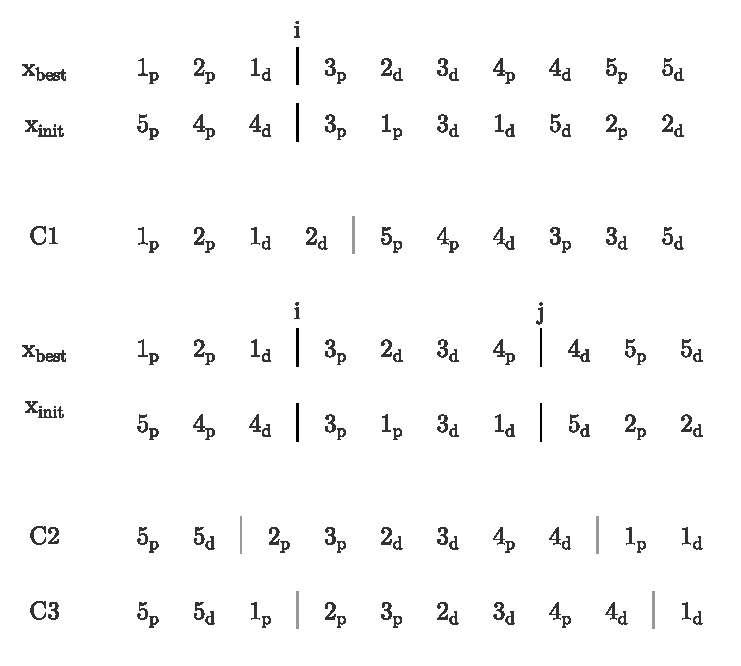
\includegraphics[width=0.9\textwidth]{figures/crossover.pdf}
        \caption{A visualisation of the three crossover operators.}
        \label{fig:crossover}
    \end{figure}
    
    \begin{description}
    		
    		\item [One-point Crossover (C1)] This operator is inspired by Prins (2004) \cite{Prins2004}, who applied this operator to instances of classical VRP. In our usecase of PDP, the operator works as follows: first, a random position $i$ is selected, such that $0 < i < \max_{k \in K}{|e_k|}$, where $K$ is the set of drivers, $e_k$ is the route of driver $k$, and $|e_k|$ is its length. Second, all requests whose node appears before position $i$ in each route of $x_{\mathrm{best}}$ are copied to the new solution in their respective order. Finally, the rest of the requests are copied from $x_{\mathrm{init}}$ in the respective order, skipping the requests that are already in the new solution.
    		
    		\item [Two-point Crossover (C2)] A similar operator was proposed by Goldberg and Holland (1988) \cite{Goldberg1988}. In our case, two positions $i$ and $j$ are selected, such that $0 < i < j < \max_{k \in K}{|e_k|}$. The operator copies all requests, whose nodes appear between positions $i$ and $j$ in routes from $x_{\mathrm{best}}$ to the new solution while maintaining their order. Finally, the same operation is performed on nodes that appear before position $i$ and after position $j$ in routes from $x_{\mathrm{init}}$, but in reverse order.
    		
    		\item [Linear Two-point Crossover (C3)] This operator, proposed by Sevaux and Dauzère-Pérès (2003) \cite{Sevaux2003} is similar to the two-point crossover operator C2. The only difference is that after copying the nodes from $x_{\mathrm{best}}$, the rest of the nodes are copied from $x_{\mathrm{init}}$ in their respective order. After that, to ensure the precedence constraints are satisfied, a repair procedure which adds the nodes of the incomplete requests is performed.
    		
    \end{description}
    

    
    \subsection{Parameter Selection}\label{halns:parameters}
    
    The parameters mentioned throughout the algorithm description are summarized and explained in this section. Generally, the parameters are selected based on the proposals and experimental results from the literature, such as  Ropke and Pisinger (2006) \cite{Ropke2006}, Demir et al. (2012) \cite{Demir2012}, Leung et al. (2013) \cite{Leung2013}, and Masmoudi et al. (2016, 2020) \cite{Masmoudi2016, Masmoudi2020}. Three parameters were not adopted from the literature and are based on our experiments. These are the maximum number of iterations $i_{\mathrm{max}} = 100\,000$, in which we observed that the solution is no longer improving on our evaluation dataset; and the coefficients of total delay $\beta = 1$ and total distance $\gamma = 0.5$ in the cost function, which seem to be a good balance between prioritizing the user satisfaction and minimizing the operational cost. Table \ref{tab:parameters} summarizes the parameters used in our algorithm.
    
    \begin{table}[!ht]
    \centering
    {\renewcommand{\arraystretch}{1.5}
    \begin{tabular}{llll}
    \hline
    \textbf{Not.}          & \textbf{Description}                            & \textbf{Value} & \textbf{Source}             \\ \hline
    $i_{\mathrm{max}}$     & Maximum number of iterations                    & $100\,000$       &                             \\
    $\beta$                & Coefficient of delay in cost calculation        & $1$            &                             \\
    $\gamma$               & Coefficient of distance in cost calculation     & $0.5$          &                             \\
    $n_{seq}$              & Num. of iterations to update the weights        & $100$          & \cite{Masmoudi2016}         \\
    $u_{min}$              & Min. \% of requests removed at each iteration   & $0.175$        & \cite{Pisinger2007}         \\
    $u_{\mathrm{max}}$     & Max. \% of requests removed at each iteration   & $0.35$         & \cite{Pisinger2007}         \\
    $r_p$                  & Roulette wheel parameter                        & $0.7$          & \cite{Masmoudi2016}         \\
    $P^0_{r}$              & Initial probability of removal operators        & $0.1$          & \cite{Masmoudi2016}         \\
    $P^0_{i}$              & Initial probability of insertion operators      & $0.125$        & \cite{Masmoudi2016}         \\
    $P^0_{ls}$             & Initial probability of local search operators   & $0.125$        & \cite{Masmoudi2016}         \\
    $\pi_{1}$              & Score of a new best solution                    & $15$           & \cite{Masmoudi2020}         \\
    $\pi_{2}$              & Score of a new current solution                 & $10$           & \cite{Masmoudi2020}         \\
    $\pi_{3}$              & Score of a feasible non-improving solution      & $5$            & \cite{Masmoudi2020}         \\
    $\tau_{\mathrm{max}}$  & Initial temperature                             & $25$           & \cite{Leung2013}            \\
    $\alpha$               & Cooling rate                                    & $0.99975$      & \cite{Ropke2006, Demir2012}

    \end{tabular}
    }
    \caption{The parameters used in our HALNS algorithm}
    \label{tab:parameters}
    \end{table}
    
\section{Methods for Evaluation}
    
    To evaluate the performance of the HALNS algorithm described in the previous section, three important components were needed. Firstly, we created datasets with different instances of the problem, i.e., with different number of requests and drivers. Secondly, we constructed a baseline algorithm for comparison with the newly developed HALNS algorithm. Lastly, we defined the metrics to be used for evaluating both the baseline and the HALNS algorithms.

    \subsection{Evaluation Datasets} \label{sec:dataset}
    
    Evaluation datasets contain different sizes of the problem instances. To create these datasets, we used real data from a selected company, which delivers food from seven restaurants in Prague. The data that could match the order details to specific customers were removed to keep anonymity.
    
    For each request, the collected data relevant to our purposes are the following:
    
    \begin{enumerate}
        \item Pickup Location
        \item Drop-off Location
        \item Pickup Time Window
        \item Drop-off Time Window
        \item Order Creation Time
        \item Number of Packages
    \end{enumerate}

     To create the different instances, we took all requests from this company since the 1\textsuperscript{st} of January 2020 until the 5\textsuperscript{th} of May 2020, totalling 7\,100 requests. Next, all time windows of these requests were shifted to a single day. Figure \ref{fig:dataset-map} shows a distribution of the coordinates on the map of Prague. The distribution of the starts of the time windows at drop-off locations of these requests is shown in figure \ref{fig:dataset-distribution}. It is clear that the vast majority of all deliveries should be delivered between 11 AM and 1 PM.
    
    \begin{figure}[!ht]
        \centering
        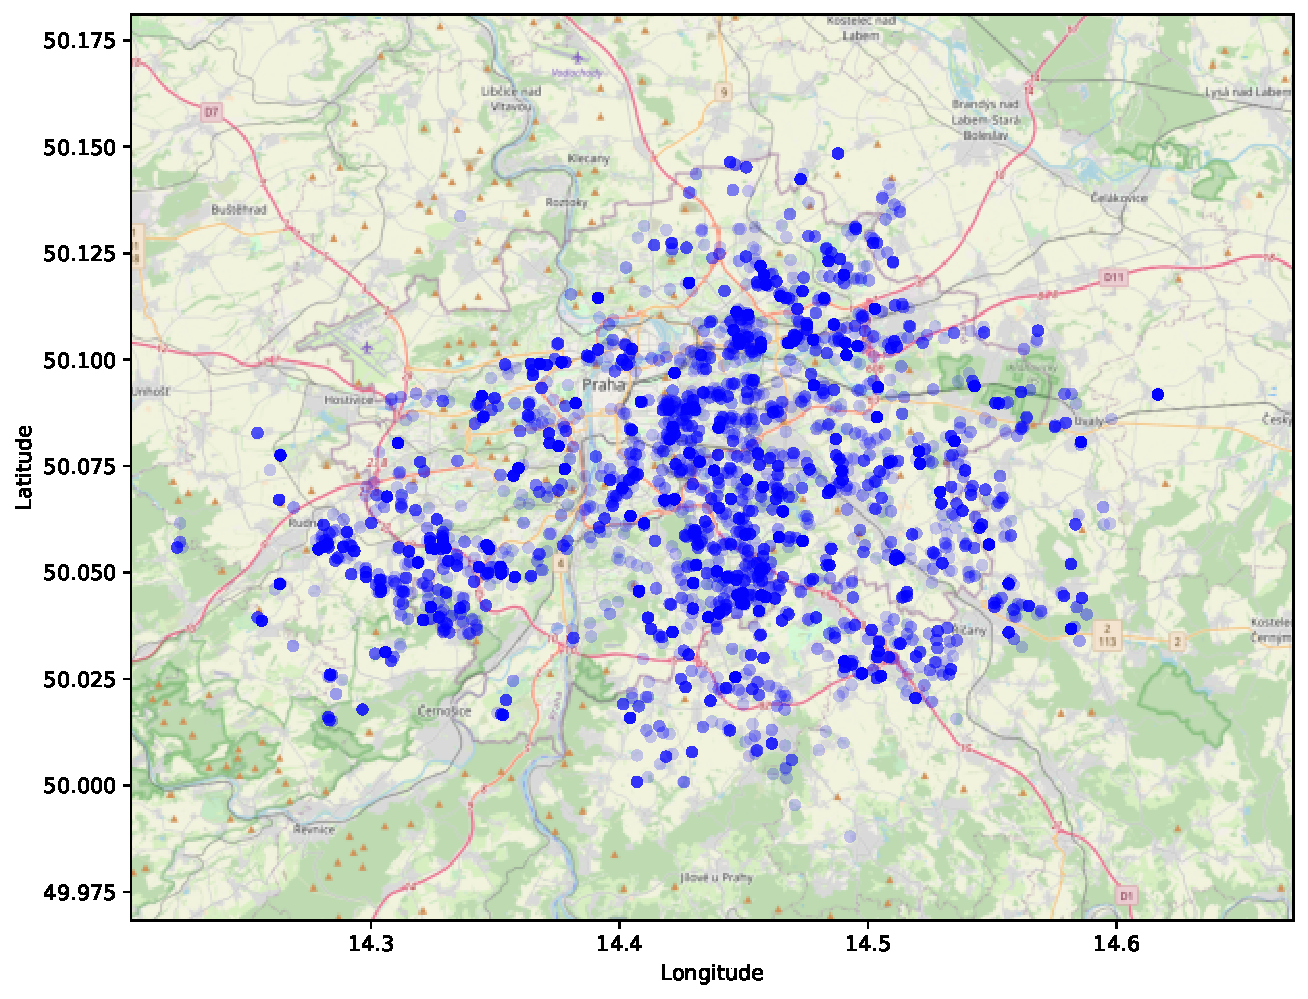
\includegraphics[width=\textwidth]{figures/dataset-map.pdf}
        \caption{A distribution of drop-off locations in the full request dataset of 7\,100 requests.}
        \label{fig:dataset-map}
    \end{figure}
    
    \begin{figure}[!ht]
        \centering
        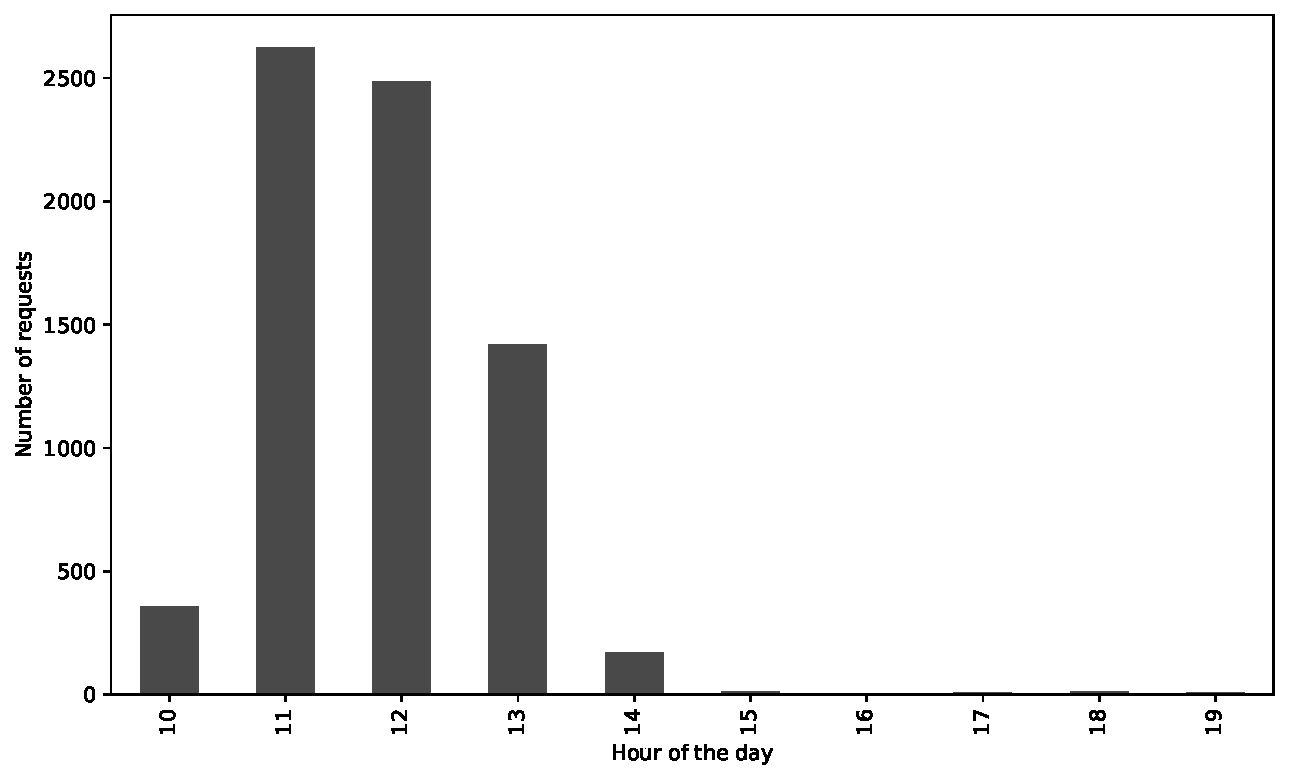
\includegraphics[width=\textwidth]{figures/dataset-distribution.pdf}
        \caption{A distribution of the earliest times of drop-off set by the customers throughout the day in the full request dataset of 7\,100 requests.}
        \label{fig:dataset-distribution}
    \end{figure}

    The individual instances were created by selecting random subsets of different sizes from this set. We used five different instance sizes and prepared 10 instances of each size. For each of these instance sizes, the number of drivers was determined. Based on the distribution of time windows in figure \ref{fig:dataset-distribution}, most requests arrive in a period of 2.5 hours. Additionally, based on our experiments with our current ORTools planner, a single driver is able to finish 3.5 requests per hour. Thus, the number of drivers is computed as $\mathrm{round}(\frac{|r|}{2.5\,3.5})$, where $|r|$ is the number of requests in the instance.
    
    To sum up, 10 different random instances of each of the following sets were prepared. They are shown in table \ref{tab:datasets}.
    
    \begin{table}[!ht]
    \centering
    {\renewcommand{\arraystretch}{1.5}
    \begin{tabular}{lll}
    \hline
               & \textbf{Requests} & \textbf{Drivers} \\ \hline
    \textbf{1} & 20                & 2                \\
    \textbf{2} & 50                & 6                \\
    \textbf{3} & 100               & 11               \\
    \textbf{4} & 200               & 22               \\
    \textbf{5} & 500               & 56              
    \end{tabular}}
    \caption{5 evaluation datasets, each containing 10 different instances}
    \label{tab:datasets}
    \end{table}

    
    \subsection{Baseline Algorithms} \label{sec:baseline}
    
    As a baseline, three methods were used. The first is a simple insertion heuristic, as was used for constructing an initial solution for the HALNS algorithm and is described in section \ref{halns:init-solution}. The second is the ORTools planner that is already part of the GoDeliver system and is described in section \ref{sec:godeliver-current-state}. The last one combines the insertion heuristic with the ORTools planner, first creating the solution using the insertion heuristic, and using that solution as an initial solution for the ORTools planner for improvement. This approach overcomes the problem that ORTools is unable to find an acceptable solution on larger instances. These three methods are visualised in figure \ref{fig:baseline-algorithms}.
    
    \begin{figure}[!ht]
        \centering
        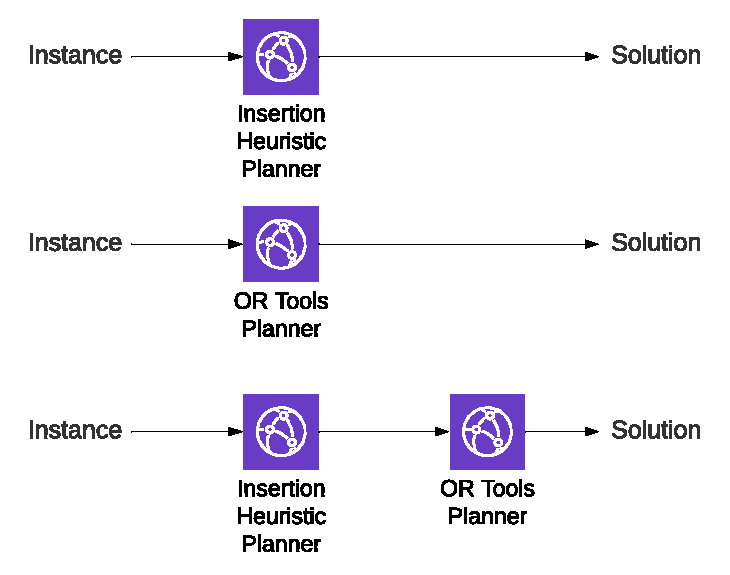
\includegraphics[width=0.8\textwidth]{figures/baseline-algorithms.pdf}
        \caption{Three baseline algorithms for evaluating the performance of our HALNS algorithm.}
        \label{fig:baseline-algorithms}
    \end{figure}
    
    \subsection{Metrics} \label{sec:metrics}
    
    For problem instances of more than a few tens of requests, it is nearly impossible to find the optimal solution. In addition, the cost of the solution alone does not reveal the full information about the solution quality. For these reasons, we defined the metrics that help us evaluate the solutions produced by different algorithms. These metrics indicate how good the produced solutions are with respect to our objectives.

    These metrics include:
    \begin{description}
        \item[Delay of Drop-off (M1)] This is probably the most important metric that best describes the customer satisfaction constraint. It indicates the time difference between the drop-off time window and the estimated time of arrival of the drivers. We measure the average and the maximum delay per request. 
        
        \item[Total Distance Travelled (M2)] This is the second most important metric which shows the optimality of the routes with respect to the cost of delivery. It is defined as the sum of the total distance travelled by all drivers.
        
        \item[Total Time Spent (M3)] This metric is an addition to the previous metric M2. It indicates the total time spent on the route across all couriers. We assume a high correlation between this metric and the M2 metric, since the distance is directly proportional to the driving time. However, this metric also includes the waiting times at the nodes and thus might produce different results.
                
        % \item[Delay of Pickup (M4)] Similarly to the M1 metric, we measure the time difference between the pickup time window and the estimated time of arrival of the drivers. This metric does not relate too much to customer satisfaction, but contributes to the wuality of the service.

        % \item[Number of Deliveries per Driver (M4)] This metric indicates how many requests were handled by a single driver. While the average will always be the same, i.e., $|r|/|K|$, where $|r|$ is the number of requests and $|K|$ is the number of drivers, the maximum and minimum numbers can reveal either insufficient or excessive number of drivers.
        
        \item[Delivery En Route Time (M4)] This metric shows the duration of a single delivery between its pickup and drop-off estimated times. In other words, it shows how long is the delivery (in our case the food) in the vehicle before it is delivered. This is especially important for perishables, such as ready-to-eat meals.
        
        \item[Delivery Load (M5)] This metric indicates how well the algorithm is able to stack the requests within the route, i.e., it is the average number of orders picked up by the driver at one location.
        
    \end{description}

\section{Implementation}
    
    This section describes the implementation details of the planning algorithm and its integration into GoDeliver pipeline. It also briefly illustrates the developed evaluation environment that is also part of this thesis.
    
    \subsection{Planning Algorithm}
    
    The main HALNS algorithm described in section \ref{sec:halns} as well as the insertion heuristics baseline mentioned in section \ref{sec:baseline} were implemented in \emph{Go} language\footnote{\url{https://golang.org/}} version \emph{1.15.8}. We opted for Go primarily for these reasons: it is a statically typed, compiled language and thus much more performant compared to, for example, Python; it has great support for concurrency which allows to speed up the algorithm even more; it is easy to create compiled binaries for all operating systems which makes the continuous integration pipeline easy; and finally there is a large community around Go which contributes to our confidence in its further development and support.
    
    The most critical entity in the whole algorithm is the \texttt{solution} structure that is constantly being destroyed by removal operators, repaired by insertion operators, improved by the local search procedure, and combined with a new solution by applying the crossover mechanism. The solution instance keeps the list of $n$ \texttt{plans}, where $n$ is always the required number of drivers, and a set of unplanned \texttt{requests}, i.e., the requests that are not part of the solution, for example, after the removal operator is applied. Each plan contains a list of \texttt{actions}. Actions represent the graph nodes of a specific type. An action can be of three types: start, pickup, and drop-off. Each request contains one or two actions, depending on whether the request is already picked up before the planning procedure starts (see section \ref{sec:dynamicity}). In the static variant, a single request contains exactly two actions: pickup and drop-off. For better understanding, figure \ref{fig:entity-diagram} reveals the relationships between these entities.
    
    \begin{figure}[!ht]
        \centering
        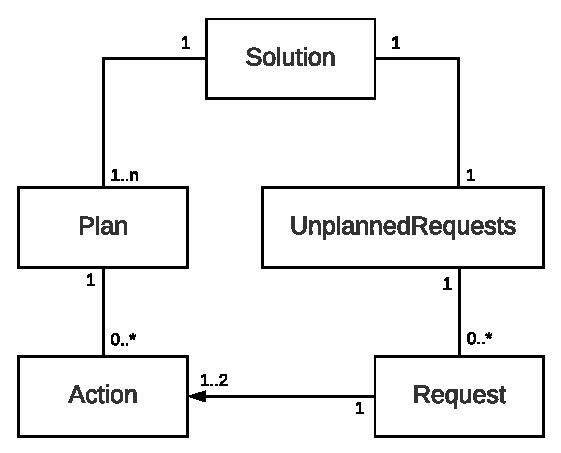
\includegraphics[width=0.6\textwidth]{figures/entity-diagram.pdf}
        \caption{A simplified entity relationship diagram of the data model used in Go implementation.}
        \label{fig:entity-diagram}
    \end{figure}
    
    
    Because Go works with the concept of interfaces rather than inheritance, so typical for other languages, the architecture of the algorithm is notably shaped by this concept. We define four interfaces for the operators used: removal, insertion, local search, and crossover. Each of these interfaces defines a different signature for the \texttt{Apply} method, that applies the operator and produces a new solution. For example, the removal operators accept two parameters: the current solution and the number of requests to remove, whereas the crossover operators need to be provided with two solutions as parameters. These interfaces are shown in figure \ref{fig:operators-diagram}.

    
    \begin{figure}[!ht]
        \centering
        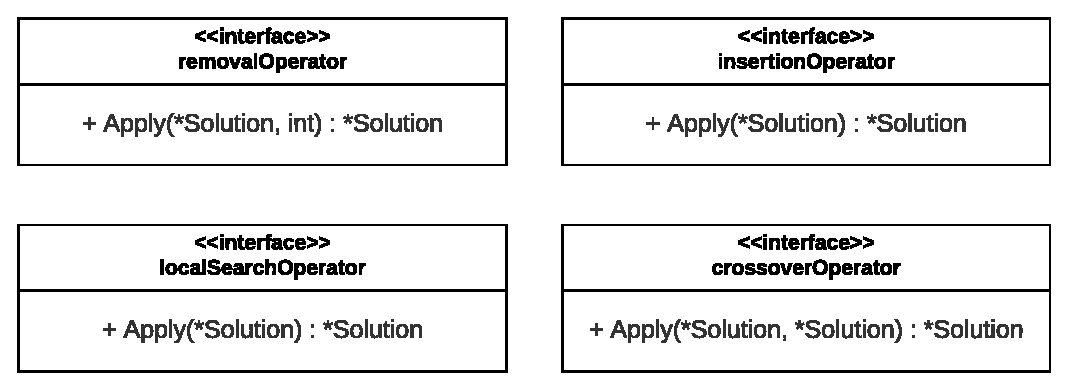
\includegraphics[width=0.8\textwidth]{figures/operators-diagram.pdf}
        \caption{Four operator interfaces used in the Go implementation of the HALNS algorithm.}
        \label{fig:operators-diagram}
    \end{figure}  
    
    \subsection{Integration into GoDeliver Pipeline}
    
    Extensive work was done on the integration part. The previous state of the GoDeliver Planner Service is described in section \ref{sec:godeliver-current-state}. The service was tightly coupled with the ORTools solver and was not extendable nor easily testable. Therefore, we abstracted the individual planning algorithms (baseline and HALNS) into their respective classes, which extend the \texttt{AbstractPlanner} class. This class is now responsible for serializing the instance, calling the respective planner, and deserializing the solution. Since the HALNS and insertion heuristics planners are implemented in Go, the GoDeliver Planner Service loads an already compiled binary as a C library, which can be called from Python. The class diagram of \texttt{AbstractPlanner} class and its subclasses is shown in figure \ref{fig:abstract-planner-diagram}.
    
    \begin{figure}[!ht]
        \centering
        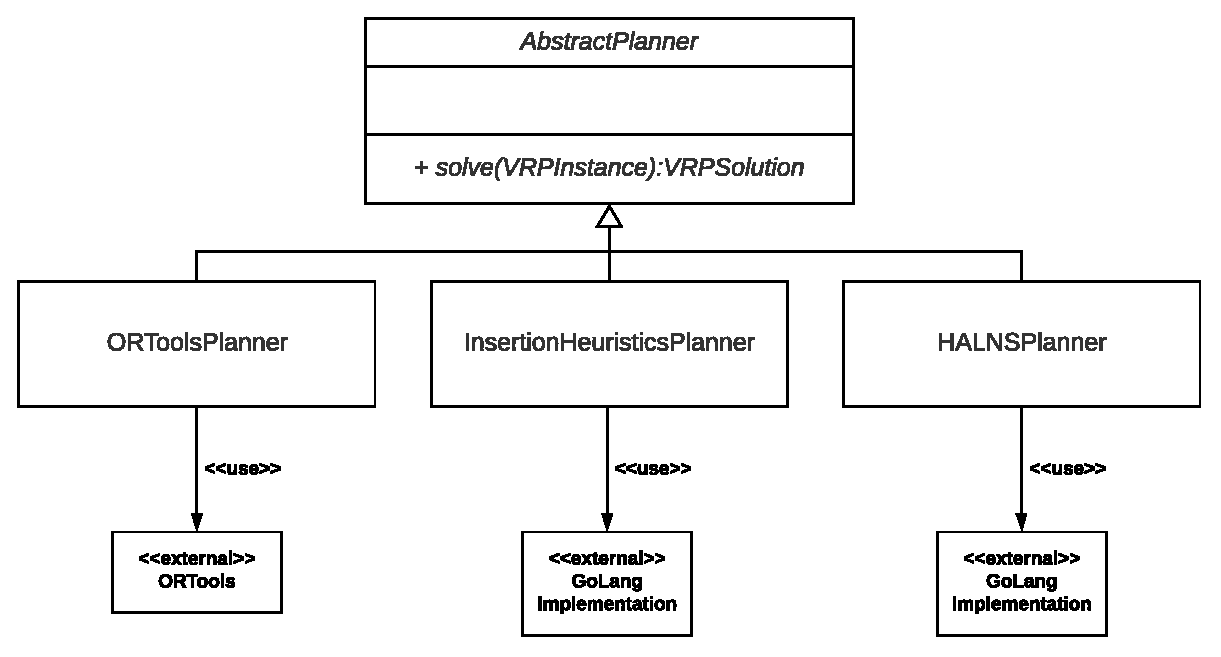
\includegraphics[width=0.8\textwidth]{figures/abstract-planner-diagram.pdf}
        \caption{The Abstract Planner class, and three specific planner implementations in GoDeliver Planner.}
        \label{fig:abstract-planner-diagram}
    \end{figure}  
    
    In addition to this abstraction, we introduced a way to easily benchmark these planning algorithms and visualize the produced solutions and metrics. For that, we use \emph{plotly}\footnote{\url{https://plotly.com/}} framework for visualizing the plans and \emph{streamlit}\footnote{\url{https://streamlit.io/}} framework that displays the metrics of all methods in a simple and understandable way. Figure \ref{fig:godeliver-architecture-new} displays the improved and extensible architecture of GoDeliver Planner Service.
    
    \begin{figure}[!ht]
        \centering
        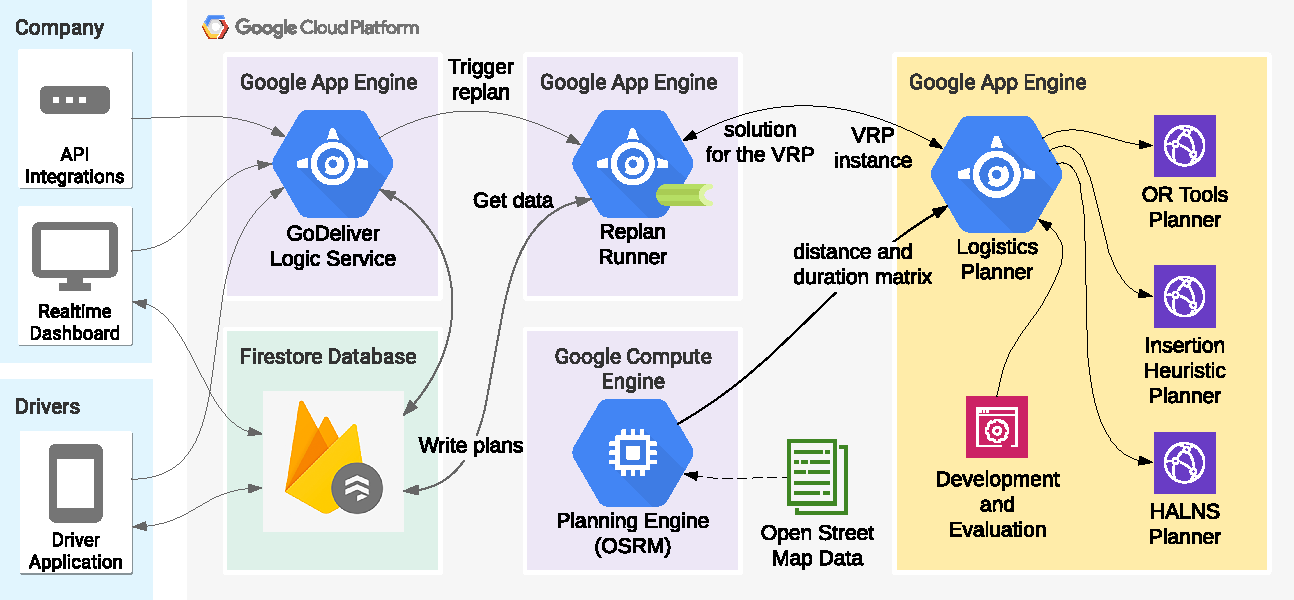
\includegraphics[width=1\textwidth]{figures/godeliver-architecture-new.pdf}
        \caption[The new architecture of GoDeliver Planner.]{The new architecture of GoDeliver Planner (highlighted by the yellow rectange).}
        \label{fig:godeliver-architecture-new}
    \end{figure}
    